\documentclass[onecolumn]{preport}
\usepackage[dvipdfmx]{graphicx}
\usepackage{comment}
\graphicspath{{figs/}}

\title{CNC切削加工入門}
\author{文責:ワッシャー (twitter:@ntm510)}

\begin{document}

\pagestyle{empty}
\maketitle
\thispagestyle{empty}
\sloppy

\begin{comment}
\section*{初めに}

本稿はプログレスレポートのテンプレートである\cite{Sakai}.

本稿における「、」や「。」は、\verb|make pub|を実行することで、「,」や「.」に変更される。

図は\figref{nowprinting}や\tabref{sample}として参照する.

\begin{figure}[tbh]
 \begin{center}
  \begin{minipage}{0.3\columnwidth}
   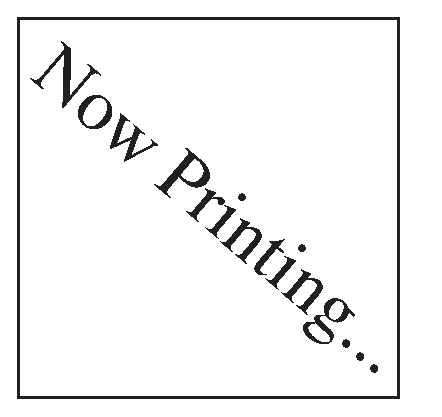
\includegraphics[width=\columnwidth]{nowprinting.eps}
   \caption{eps図の参考例}
  \end{minipage}
  \hspace{0.15\columnwidth}
  \begin{minipage}{0.3\columnwidth}
   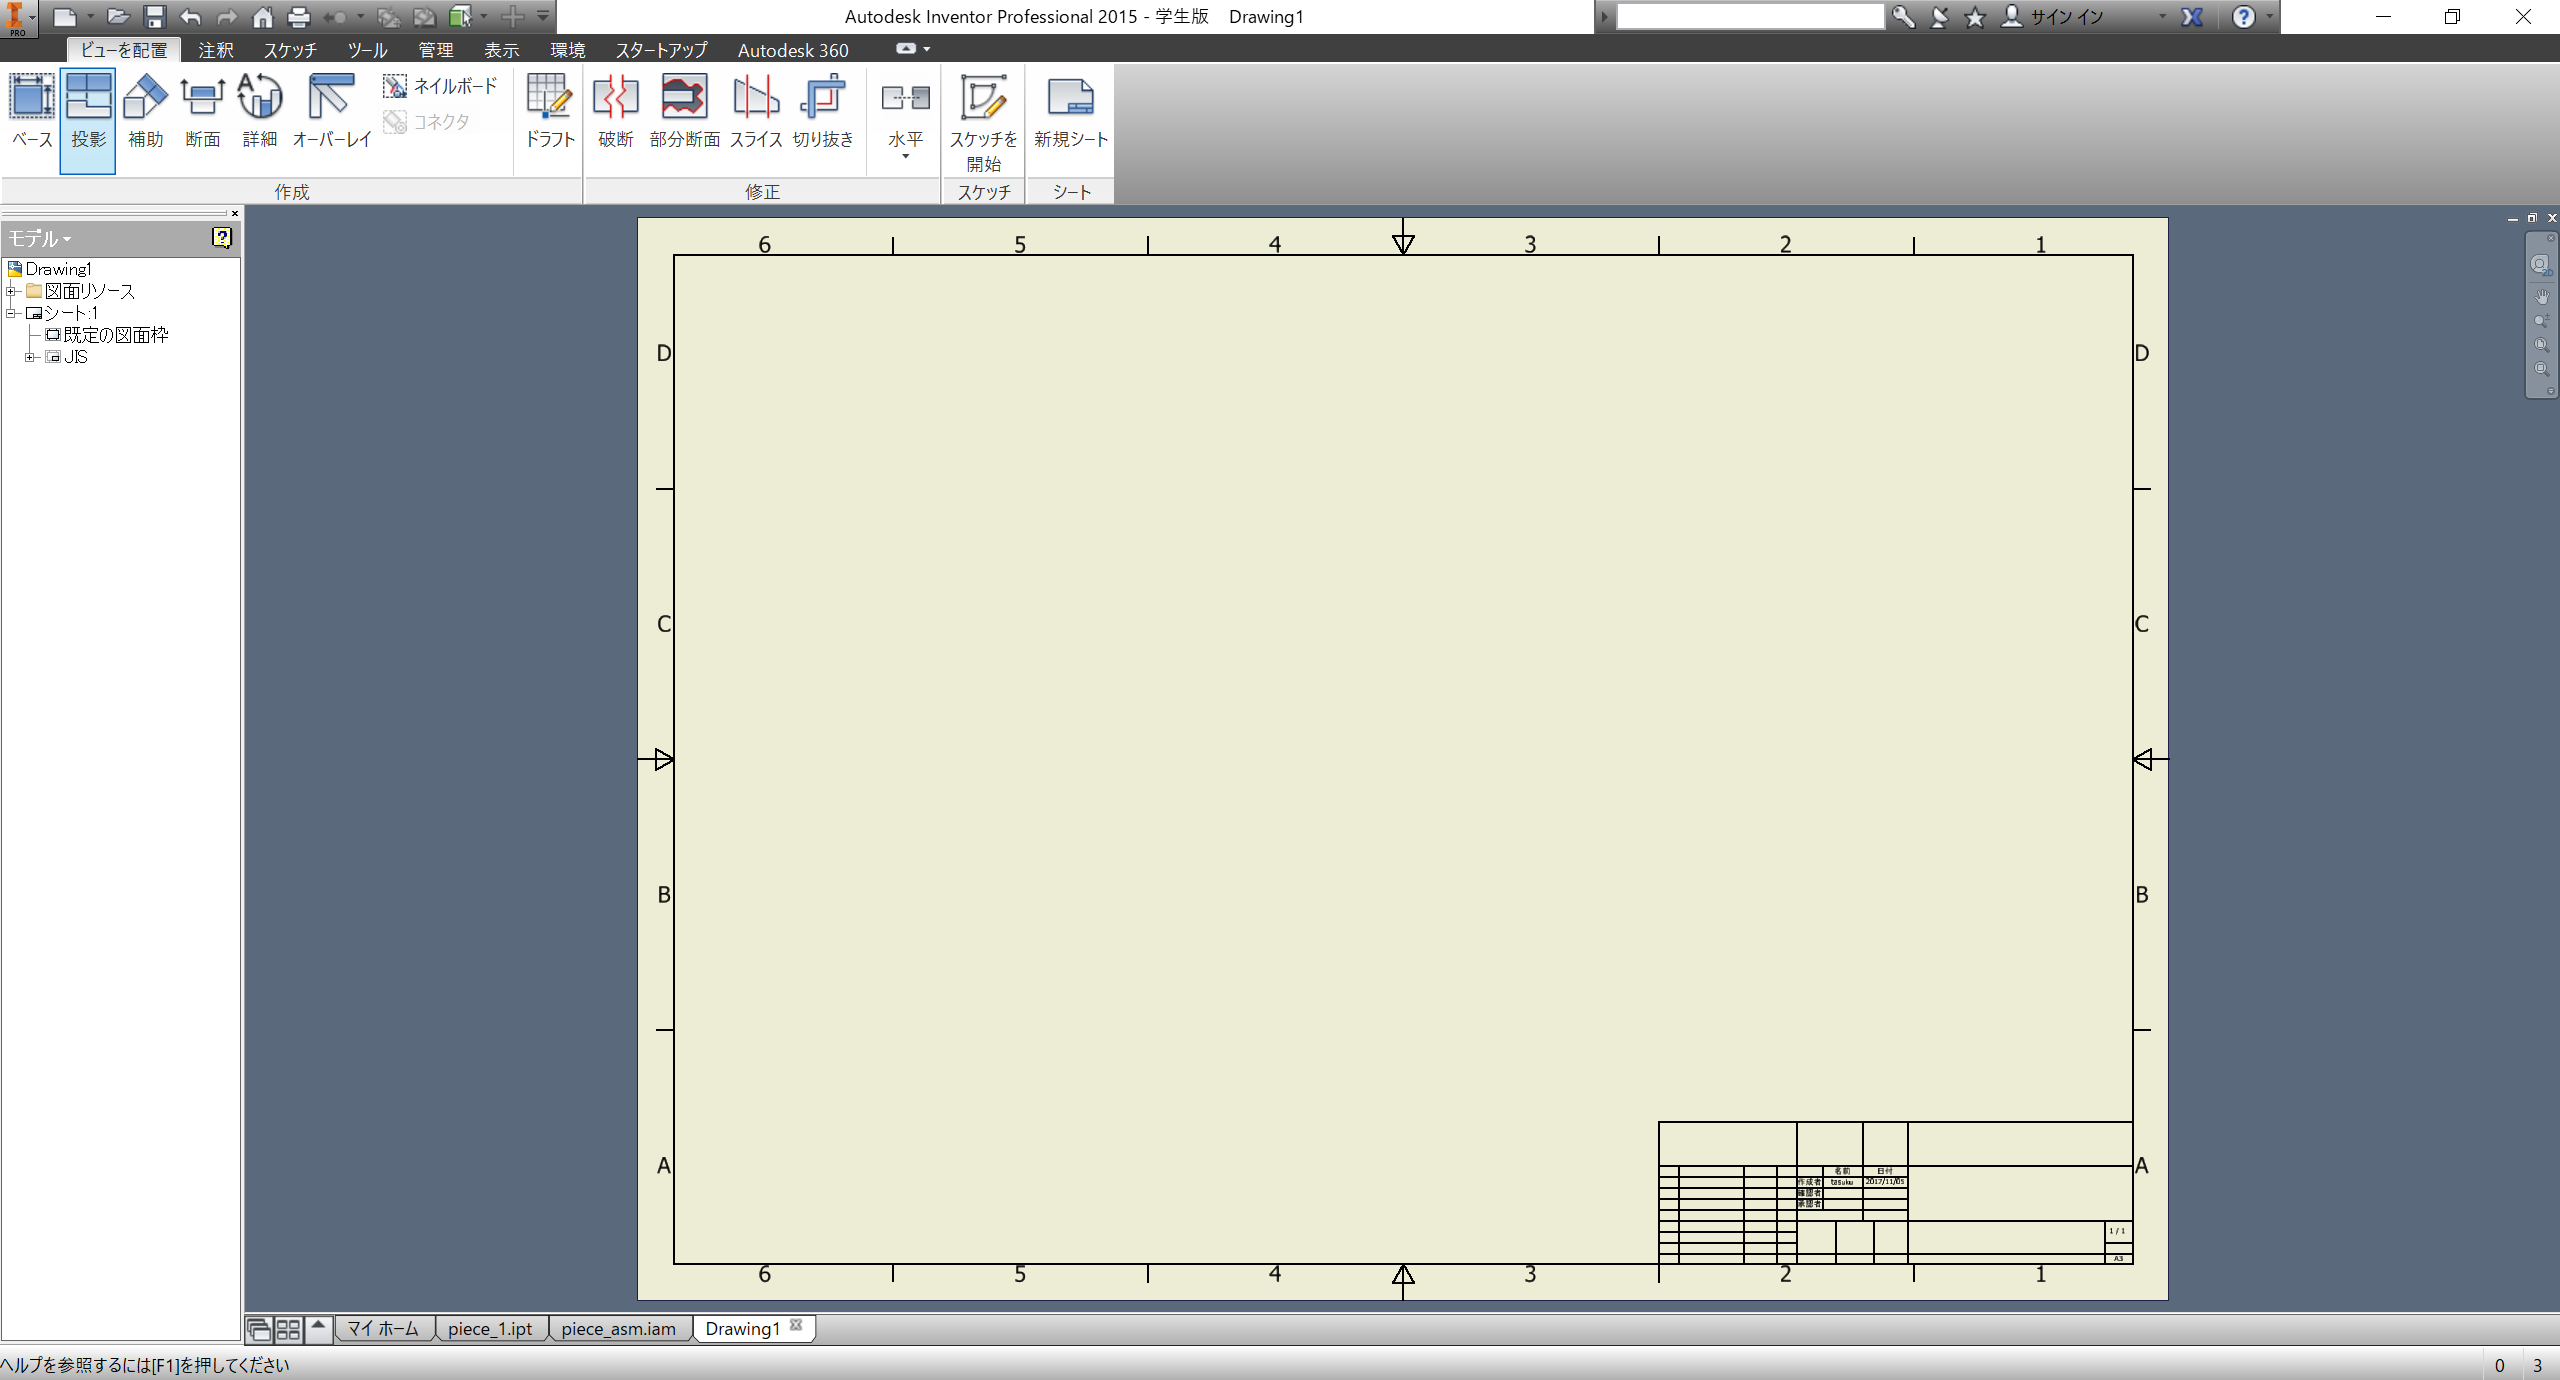
\includegraphics[width=\columnwidth]{plane.png}
   \caption{jpg図の参考例}
  \end{minipage}
  \label{figure:nowprinting}
 \end{center}
\end{figure}

\begin{table}[tbh]
 \begin{center}
  \begin{tabular}{|l|r|} \hline
  A1 & B1 \\
  A2 & B2 \\ \hline
  \end{tabular}
  \caption{図の参考例}
  \label{table:sample}
 \end{center}
\end{table}

\section{各種タイトルでどうしても改行が必要 となる場合の対処法について}

\verb|\section, \subsection|などで改行をしたい場合は単語の間にスペースを入れる。

\section{おわりに}

\bibliographystyle{junsrt}
\bibliography{p-report}
\end{comment}

\part*{始めに}

他の人にCNCなどの切削加工機の使い方を教える時などに、体系的にまとまった資料がなくて困ったことが多くあったので、この機会にまとめて文章することでそういう人への資料にしつつ、せっかくなので同人誌に加えてもらおうと思って書きました。特殊な事項も多いと思うので、それぞれ読み替えてください。あと、本当に基本中の基本しか書いていないので、応用的なことを行いたい場合はその辺のCNC切削が好きな人(この同人誌を買うような人の周りにはどうせいると思います)に聞いてみてください。気になる点とか誤字脱字があったらtwitterのDMにでも送ってくれると筆者が喜びます。

\part{知識編}

まずは基本的な知識について記述します。ここでは、切削に用いるエンドミルと、切削される側の材料について説明します。

\section{エンドミルの基本}

\subsection{エンドミルの種類}

エンドミルと一口に言っても、様々な種類があります。基本的に気を付ける必要がある要素として、1.刃の形状、2.刃直径、3.シャンク径、4.有効刃長の4つがあります。
 刃の形状とは、エンドミルの先端の形状を指します。先端が長方形になっているものをスクエアエンドミル、球状になっているものをボールエンドミルといいます。前者は切削面が平面的、後者は切削面が曲面的な加工に用いられます。ここでは前者のみを扱います。

画像1.1 スクエアエンドミル

画像1.2 ボールエンドミル

 刃直径とは、エンドミルを回転した時に先端の刃の一番外側が描く円の直径を指します。これによって切削が可能な幅と、回転軸からどの程度の距離の範囲が切削されるかが決まります。例えば刃直径が3mmのエンドミルの場合、エンドミルの中心が通った直線を中心とした、幅3mmの領域が切削されます。また、直径が大きいと切削領域が大きくなるため、基本的に切削時間は短くなります。ポケット加工(後述)など、切削領域が大きく時間がかかる場合は、影響が出ない範囲で大きなエンドミルを使うと加工時間の短縮が図れます。

画像2 スクエアエンドミルの底面の画像

 次に、シャンク径とは、エンドミルのうち刃のついていない上部の円筒状の部分の直径のことであり、写真のエンドミルの場合Φ4となっています。普段よくCNCで使われる程度のサイズだと、4mm,6mm,10mmなどが一般的です。
 最後に、有効刃長とは、エンドミルのうち切削が可能な長さのことで、これと等しい長さだけ深く切削を行えます。例えば、上の写真のエンドミルについては、有効刃長が8mmのため、厚みが8mmまでの板材であれば基本的に問題なく切削が行えます。しかし、それ以上の厚みの板材だと、刃が無いシャンク径が4mmの部分までエンドミルを挿し込むことになり、シャンクと刃の間のテーパー部分が板材に接触して事故の原因になります。有効刃長を超えた切削はCNCの故障の原因になるため、使用の際には十分に注意をしましょう。

画像3 スクエアエンドミルの横からの画像

\subsection{ダウンカットとアップカット}

ダウンカットとアップカットは、被切削材に対しエンドミルの回転方向と切削方向がどのようになっているかを表しています。ダウンカット(下向き削り)とは、工具の刃が未切削の部分に当たって材を削り下げる削り方、アップカット(上向き削り)とは、工具の刃が切削済みの部分に当たって削りあげる削り方を指します。ダウンカットでは切り込み時が最も材への食いこみが大きく次第に小さくなり最終的に0になるのに対し、アップカットでは食い込みが最初は0で次第に大きくなります。詳細は省きますが、びびりや摩擦熱が生じて工具寿命が短くなるなどの理由から、基本的にCNC加工の際はダウンカットで加工を行います。通常、エンドミルの回転方向は正転(上からみて時計周り方向)にであるため、外形カットを行う場合エンドミル自体の経路も時計回りになります。

画像4 ダウンカットアップカットとかの図を作って張る

\subsection{エンドミルの固定方法}

 エンドミルの固定方法には、1.いもねじ,2.ドリルチャック,3.コレットの3種類ほどが一般的です。
 いもネジによる固定は特に書くことはありません。カップリングなどと同様に留めれば大丈夫ですが、六角ねじの穴が死にやすいので過度に力を入れて締めすぎないようにしましょう。
 ドリルチャックについても、一般的なボール盤のドリルのチャック方式と同じです。チャックハンドルはサイズの合ったものを使いましょう。また、ボール盤でも同様ですが、まれにチャックハンドルを付けたままエンドミルを回してチャックハンドルを吹き飛ばす事故が起きるので、気を付けましょう。当たると痛いです。
 最後にコレットによる固定です。主にATC付のCNCでエンドミルを使用する際などに使います。スリットの入った紡錘形の金属部品の中心にエンドミルを挿し、周りを締め付けることで固定を行います。詳しくはユキワ精工のHPなどを参照してください。
 どの固定方法にしても共通で気を付けることとしては、切削をする材の上面がきちんとZ軸方向の原点位置に来るようにすることです。エンドミルを材に自重で接触させた上でチャックを行うなどの方法が簡単です。エンドミルの先端に前回の加工の削りカスや、材の固定用の両面テープの粘着部分などが付いていると、最初の固定の際にエンドミル原点がZ軸上方向にずれるため、削り残しが出てしまうことがあります。加工のたびにエンドミルをパーツクリーナーなどできれいにしましょう。

画像5 固定部分の画像、何か適当に

\section{材料の基本}

 材料としてよく用いられるものとして、樹脂と金属があります。

\subsection{樹脂}

 主に用いられる樹脂材として、アクリル樹脂,ABS,POM,ポリカーボネート,MCナイロンなどが挙げられます。全般的に言えることとして、厚み方向が厳密ではない場合があることに注意が必要で、例えばt5で売られている板の実寸の厚みがt5.7だったりします。ここではそれぞれの特徴について記述します。

\subsubsection{アクリル樹脂}

 樹脂板の中でも安価で、透明で見た目が綺麗なこと、レーザー加工が綺麗に行えること、アクリル用接着剤で溶着が容易なことが利点です。ただし衝撃に弱く、割れる時にはパキっと割れるので、ギヤなど機械的強度が必要な
場合にはお勧めしません。

\subsubsection{ABS}

 アクリルの次に安価で、アクリルより機械的強度が高いです。樹脂の中でも融点が低めで、融けてエンドミルにへばりつきやすいので、加工する速度に注意が必要です。レーザー加工も可能ですが、切断面がアクリルより粗くなりがちです。また、融点が低いことから3Dプリンタのフィラメントに良く使われます。

\subsubsection{POM}

 滑りが良いので、摺動部などに向いています。レーザー加工も可能で、アクリルの次に綺麗に切れます。機械的強度も高めで、色々と手ごろでちょうどよいため、使いやすい素材です。撃力で割れることもあるので過信は禁物です。

\subsubsection{ポリカーボネート}

 POMよりも機械的強度が高く粘り強いため、衝撃があってもそうそう割れないという特徴があります。加えて、アクリル用接着剤での溶着も容易となっています。加工性はABSやPOMなどより劣るため、注意が必要です。また、加工の際に除去しにくいバリが残るという点もあります。見た目がアクリルと近いのですが、異なる特徴として弾性がアクリルより強いことと、断面が少し青みがかっていることがあげられます。

\subsubsection{6ナイロン}

 MCナイロンとも呼ばれる、既製品の樹脂ギヤにも用いられる樹脂材です。機械的強度はこの中では最も高いですが、ポリカーボネートと同様にバリが除去しにくいことと、価格が高価なことが良くない点として挙げられます。また、吸湿して膨張するという特徴もあるため、例えば長い梁のようなパーツを作ると、ものすごくたわむので注意が必要です。

画像6 融点、レーザー加工可能性、バリの取りやすさ、価格、ヤング率、比重などの表

情報元のURL

樹脂:http://www.kda1969.com/

\subsection{金属}

 金属を用いる理由としては、一番に重量当たりの強度で樹脂より優れていることがあげられます。

\subsubsection{アルミ合金}

 アルミ合金と一口に言っても、、色々と種類があります。筆者がよく使っていたのはA5052(板材)やA6063(角パイプ)などです。型番の意味は以下のようになります。ここでは、A5052,A2017(ジュラルミン),A2024(超ジュラルミン),A7075(超々ジュラルミン)を紹介しますが、CNC加工では基本的にA5052を用います。たわみなどが心配な場合は、CADに付属しているCAEで計算した上で、必要なヤング率を満たすものを使用しましょう。ちなみに、ヤング率で比較を行うと、工作用アルミ<ジュラルミン<超々ジュラルミン<ジュラルミン<超ジュラルミンとなります。特にこだわりがなければ、基本的に工作用のA5052が入手しやすそうです。厚みについては、ぴったり寸法の通りであることが多いようです(購入している業者によるのかは筆者のリサーチ不足です)。通常のCNC加工ではA5052を使うのが良いでしょう。

アルミの型番と種類
1000番台:純アルミ 
2000番台:Al-Cu系(ジュラルミン、超ジュラルミンはここ)
3000番台:Al-Mn系
4000番台:Al-Si系
5000番台:Al-Mg系(工作用アルミ材はここ)
6000番台:Al-Mg-Si系
7000番台:Al-Zn-Mg系(超々ジュラルミンはここ)

アルミの種類とヤング率(単位はGPa)
A5052(工作用アルミ):70.6
A6063(角パイプ):68.6
A2017(ジュラルミン):72.6
A2024(超ジュラルミン):73.5
A7075(超々ジュラルミン):71.6

アルミの種類と比重(単位はg/cm\verb|^|3)
A5052(工作用アルミ):2.79
A6063(角パイプ):2.70
A2017(ジュラルミン):2.75
A2024(超ジュラルミン):2.78
A7075(超々ジュラルミン):2.81

アルミ:http://www.alumitech.co.jp/html/download5.html

\subsubsection{真鍮}

 真鍮の中でもよく用いられるのがC3604(快削真鍮)です。入手性が良く、比重が高い金属の中では加工性が良いため、フライホイールや重りなどの重量物を作る際に向いています。後は、樹脂材との滑りが比較的良いため、溝カムなどの摺動部に用いることもあります。
 
\subsubsection{鉄(ステンレス含む)}

 入手が容易な金属の中でも加工が比較的難しく、加えて重いので、荷重が大きくかかる軸など、ロボコン用途では一部の機械的強度が重要なパーツを除いてあまり多くは使われない印象です。CNCでも加工できないことはないですが、長い時間と大量の切削油とエンドミルの犠牲が必要なため、お勧めしません。

\subsection{その他}

 樹脂でも金属でもない材料をその他とします。

\subsubsection{MDFボード}

 Midium Density Fiber Boardの略で、中密度繊維板とも呼ばれるもので、木の繊維を樹脂で板状に固めて作られています。基本的にレーザーで加工を行う材料であり、筆者はt4のものを頻繁に使います。加工が容易な上に木工用ボンドで接着が容易なため、さっとプロトタイピングを行うときには非常に便利です。切削での加工も可能ですが、加工時間などの観点からレーザーで加工されがちです。また、強度は樹脂や金属より当然劣り、また材質が木材に近いことからへこみなども生じやすいため、そもそも厳密な寸法が必要な部品の作成には不向きです。
         
\part{実践編}

 ここからを実践編とします。具体的には、
工程1.inventorでの部品設計、vector形式ファイルの作成
工程2.CAMソフト(Cut2D)でのツールパス設計
工程3.CNCでの作業、清掃
という順番で切削部品の製作を行います。
 まず工程1では、CADによる部品の設計と、経路設計に必要な外形線を含むvector形式ファイルの作成を行います。この工程では、製作する部品の二次元情報からvector形式ファイルを作ります。次に工程2では、工程1で作成したvector形式ファイルを元にして、実際に加工を行う経路を設計し、NCデータの作成を行います。この工程で、vector形式ファイルの調整と、切削を行う深さ情報を加えた三次元のツールパスの設計を行います。最後に工程3では、工程2で設計したNCファイルをCNCで読み込み、実際の切削を行います。

\section{inventorでの作業}

\subsection{基本的な部品設計}
CNCで加工が可能な部品の形状には限りがあり、基本的に底面に平行な平面またはと底面に垂直な側面の集合のみを持つ立体である必要があります。
曲面を含む場合も、前述のボールエンドミルを使えば加工は可能ですが、ここでは簡単のため説明しません。
\subsection{部品設計で気を付けること}
 CNCで切削加工を行う部品を設計する上で、エンドミルによる加工を理解する必要があります。まず第一に、切削が可能な領域は円が移動した領域であるということです。例えば、画像の設計では、外形の周囲をそのまま削ると、角の部分の内側に削り残しが生じます。そのため、円形の切り抜きをあらかじめ設計に追加しておくことで、角の部分をすべて削りきることができます。次に、エンドミル直径と等しい

\subsection{vector形式ファイルの作成}
部品の設計


\section{Cut2Dでの作業}
\subsection{経路作成の基本}
\subsection{ポケット加工}
\subsection{小ネタ}

\section{CNCでの作業}
\subsection{素材の固定}
\subsection{エンドミルの固定}
\subsection{実際の加工}
\subsection{掃除}

\part{応用編}
\section{ギヤを切削で作る }
\section{Cut2Dの便利な機能}
\section{レーザー加工機でスマホ・タブレット台を作る}

\bibliographystyle{junsrt}
\bibliography{p-report}
\end{document}
